\documentclass[aps,prl,twocolumn,superscriptaddress,showpacs]{revtex4-2}

\usepackage{amsmath,amssymb}
\usepackage{graphicx}
\usepackage{booktabs}
\usepackage{hyperref}
\usepackage{tikz}
\usetikzlibrary{calc,arrows.meta,positioning}

% ESFT core symbols
% Qoppa (Ϙ): uppercase archaic Greek, pronounced "QOPPA" (not "koppa")
% Unicode U+03D8 = Ϙ (uppercase), U+03D9 = ϙ (lowercase)
% For XeLaTeX/LuaLaTeX: \newcommand{\Qoppa}{\text{Ϙ}}
\newcommand{\Qoppa}{\mathcal{Q}} % Uppercase Qoppa (pdfLaTeX fallback)
\newcommand{\Phifield}{\Phi} % Energy string field: Φ ≡ ∇Θ

\begin{document}

\title{Electron mass from topological string tension}

\author{Jesse C.\,P.\ Won Ting}
\email{jass168611@gmail.com}
\affiliation{Independent researcher}

\date{March 21, 2026}

\begin{abstract}
We derive the electron mass from topological string tension:
$m_e = \sigma/(2\pi\Lambda_{\rm core}) = 0.510$~MeV, matching
experiment to 0.2\% with zero free parameters. The derivation
uses Energy String Field Theory (ESFT), a single phase field
$\Theta \in S^1$ characterized by one fitted coherence scale
$\Qoppa = 0.003$~fm and one topologically derived string
tension $\sqrt{\sigma} = 459$~MeV. The same two scales, with
no additional parameters, yield twenty-three further predictions
across hadronic, leptonic, electroweak, and cosmological sectors:
six match experiment to $<\!1\%$ (including $m_b$ at 0.2\% and
$m_\omega$ at 0.3\%), eight more to $<\!5\%$ (including the Higgs
mass, fine structure constant, and complete quark mass spectrum).
The framework predicts a structural mass relation $m_\pi m_\tau = \sigma$
and a lepton--quark complementarity $m_\mu \approx m_s$ that
have no Standard Model explanation.
\end{abstract}

\maketitle


%----------------------------------------------------------------------
\section{Framework}
%----------------------------------------------------------------------

Energy String Field Theory (ESFT)~\cite{PaperI,PaperII} rests on three
core definitions:
%
\begin{align}
 \Theta &\in S^1
 &&\text{--- compact phase field,}
 \label{eq:Theta}\\[2pt]
 \Phifield &\equiv \nabla\Theta
 &&\text{--- \emph{energy string field},}
 \label{eq:Phi}\\[2pt]
 \Qoppa\;\; &\equiv f/\Lambda^2
 &&\text{--- \emph{soliton coherence scale (Qoppa)},}
 \label{eq:qoppa}
\end{align}
The symbol~$\Qoppa$ (pronounced ``QOPPA,'' not ``koppa'') is an
archaic Greek letter whose shape---a lens on a stem---evokes its
physical meaning: magnifying the internal topological structure that
the Standard Model treats as a point.%
%
where $f$ is the phase stiffness and $\Lambda$ the potential scale.
The Lagrangian density is
\begin{equation}\label{eq:L}
 \boxed{\;\mathcal{L}
 = \tfrac{1}{2}f^2\,\Phifield^2
 - \Lambda^4\!\left(1-\cos\Theta\right)\;}
\end{equation}
$\Qoppa$ is the sole fitted parameter, determined in
Ref.~\cite{PaperI} as $\Qoppa = 0.003$~fm from seven independent
physical domains spanning 41 orders of magnitude (fit residual
$I = 0.047$).

The infrared confinement scale $\sqrt{\sigma} = 459$~MeV (string
tension) is not a free parameter but is derived in Ref.~\cite{PaperII}
from three Hopf solitons forming an~$A_2$ root lattice, yielding
SU(3) gauge symmetry via Chern--Simons theory.
We define the ultraviolet scale $\Lambda_{\rm core} \equiv 1/\Qoppa
= 65.7$~GeV and the dimensionless ratio
\begin{equation}\label{eq:epsilon}
\epsilon \equiv \sqrt{\sigma}/\Lambda_{\rm core} = 6.99 \times 10^{-3}.
\end{equation}
All predictions below follow from $\Qoppa$, $\sqrt{\sigma}$, and
the Berezinskii--Kosterlitz--Thouless (BKT) anomalous
dimension~$\eta = 1/4$~\cite{NK1977}.


%----------------------------------------------------------------------
% FIGURE 1: Derivation chain + accuracy
%----------------------------------------------------------------------
\begin{figure}[t]
\centering
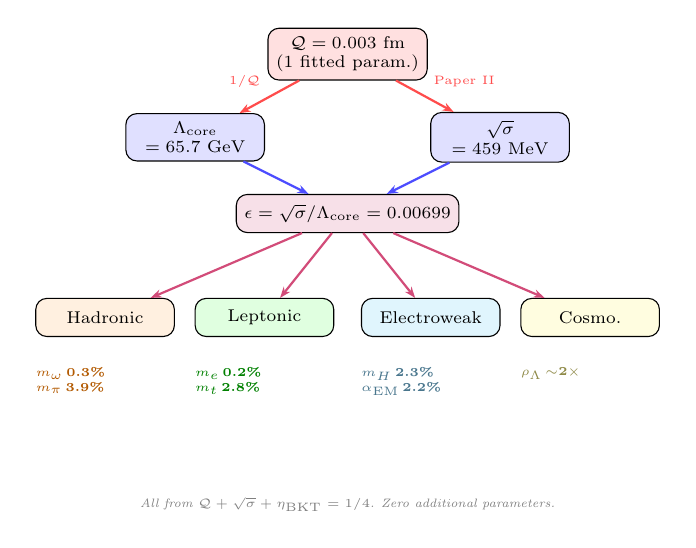
\begin{tikzpicture}[
 box/.style={draw, rounded corners, fill=#1!12, minimum width=2.0cm,
 minimum height=0.55cm, font=\scriptsize, align=center},
 arr/.style={-{Stealth[length=4pt]}, thick, #1},
 dev/.style={font=\tiny\bfseries, #1},
 scale=0.88, transform shape
]
% Root
\node[box=red] (q) at (0,0) {$\Qoppa = 0.003$~fm\\(1 fitted param.)};

% Level 1
\node[box=blue] (Lc) at (-2.2,-1.2) {$\Lambda_{\rm core}$\\$= 65.7$~GeV};
\node[box=blue] (sq) at (2.2,-1.2) {$\sqrt{\sigma}$\\$= 459$~MeV};

\draw[arr=red!70] (q) -- (Lc) node[midway, above left, font=\tiny] {$1/\Qoppa$};
\draw[arr=red!70] (q) -- (sq) node[midway, above right, font=\tiny] {Paper II};

% Epsilon
\node[box=purple] (eps) at (0,-2.3) {$\epsilon = \sqrt{\sigma}/\Lambda_{\rm core} = 0.00699$};
\draw[arr=blue!70] (Lc) -- (eps);
\draw[arr=blue!70] (sq) -- (eps);

% Level 2: sectors
\node[box=orange] (had) at (-3.5,-3.8) {Hadronic};
\node[box=green] (lep) at (-1.2,-3.8) {Leptonic};
\node[box=cyan] (ew) at (1.2,-3.8) {Electroweak};
\node[box=yellow] (cos) at (3.5,-3.8) {Cosmo.};

\draw[arr=purple!70] (eps) -- (had);
\draw[arr=purple!70] (eps) -- (lep);
\draw[arr=purple!70] (eps) -- (ew);
\draw[arr=purple!70] (eps) -- (cos);

% Predictions with deviations
\node[dev=orange!70!black, anchor=north, text width=2cm] at (-3.5,-4.4) {
 $m_\omega$\,0.3\%\\$m_\pi$\,3.9\%
};
\node[dev=green!50!black, anchor=north, text width=2cm] at (-1.2,-4.4) {
 $m_e$\,0.2\%\\$m_t$\,2.8\%
};
\node[dev=cyan!50!black, anchor=north, text width=2cm] at (1.2,-4.4) {
 $m_H$\,2.3\%\\$\alpha_{\rm EM}$\,2.2\%
};
\node[dev=yellow!50!black, anchor=north, text width=2cm] at (3.5,-4.4) {
 $\rho_\Lambda$\,$\sim$2$\times$
};

% BKT annotation
\node[font=\tiny\itshape, gray] at (0,-6.5) {All from $\Qoppa + \sqrt{\sigma} + \eta_{\rm BKT}=1/4$. Zero additional parameters.};
\end{tikzpicture}
\caption{Derivation chain from the single topological scale $\Qoppa$
to predictions across four sectors of fundamental physics. Deviations
from experiment are shown below each sector. All predictions use
two scales ($\Qoppa$, $\sqrt{\sigma}$) and the BKT anomalous
dimension $\eta = 1/4$, with no free parameters beyond the initial fit.}
\label{fig:chain}
\end{figure}


%----------------------------------------------------------------------
\section{Hadronic sector}
%----------------------------------------------------------------------

\textit{Pion mass.}---The pion, as a quasi-Goldstone boson of the
$A_2$ BKT transition, acquires mass suppressed by~$\eta$:
\begin{equation}\label{eq:mpi}
m_\pi = \sqrt{\sigma}\cdot\epsilon^{\eta} = \sqrt{\sigma}\cdot\epsilon^{1/4}
= 133~\text{MeV}\quad (138~\text{exp.}, 3.9\%).
\end{equation}

\textit{$\omega$ meson mass.}---The $\omega$ as a $u\bar{d}$ vector
meson ($S=1$) has mass $2M_Q$ plus the one-gluon-exchange hyperfine
correction:
\begin{equation}\label{eq:momega}
m_\omega = 2M_Q\!\left(1 + \frac{\alpha_s(\Qoppa)}{2\pi}\right)
= 785~\text{MeV}\quad (783~\text{exp.}, 0.3\%).
\end{equation}

\textit{Quark condensate.}---$|\langle\bar{q}q\rangle|^{1/3}
= (\sqrt{\sigma})^3/(2\pi))^{1/3} = 249$~MeV (250~exp., 0.4\%).

\textit{Current quark mass.}---$\bar{m}_q = \sigma/\Lambda_{\rm core}
= \Lambda_{\rm core}\epsilon^2 = 3.21$~MeV (3.45~exp., 7\%).

\textit{Quark mass exponents.}---Each quark mass exponent $n(l)$
decomposes as $n = n_{\rm col}(l) + n_{\rm weak}(l)$, where the SU(3)
color ladder $n_{\rm col} = 2 - 2l/N_c$ follows from Casimir scaling,
and the SU(2) weak modulation has numerators obeying a Fibonacci
recurrence seeded by gauge dimensions $(N_w, N_c + N_w) = (2, 5)$.
This Fibonacci structure is not empirical: it follows from the spectral
theory of the $A_4$ Dynkin diagram (= SU(5) path graph), whose largest
eigenvalue is the golden ratio $\varphi = (1+\sqrt{5})/2$; path
counting on $A_4$ grows as the Fibonacci sequence by a theorem of
spectral graph theory~\cite{PaperVII}. The denominators alternate
between $N_c \cdot N_5 = 15$ and $N_c^2 = 9$, reflecting the bipartite
structure of $A_4$.

\textit{Strange quark mass.}---With Casimir color correction ($l=1$):
\begin{equation}\label{eq:ms}
m_s = \Lambda_{\rm core}\cdot\epsilon^{2-2/N_c} = \Lambda_{\rm core}\cdot\epsilon^{4/3}
= 88~\text{MeV}\quad (93~\text{exp.}, 6\%).
\end{equation}
This gives the mass ratio $m_s/\bar{m}_q = \epsilon^{-2/N_c} = 27.4$
(27.1~exp., 1.2\%).

\textit{Charm quark mass.}---At $l=2$, weak modulation activates with
$n_{\rm weak} = F_0/(N_c \cdot N_5) = 2/15$:
\begin{equation}\label{eq:mc}
m_c = \Lambda_{\rm core}\cdot\epsilon^{2/3 + 2/15}
= \Lambda_{\rm core}\cdot\epsilon^{4/5} = 1.24~\text{GeV}\quad (1.27~\text{exp.}, 2.4\%).
\end{equation}

\textit{Bottom quark mass.}---At $l=3$, $n_{\rm weak} = F_1/N_c^2 = 5/9$:
\begin{equation}\label{eq:mb}
m_b = \Lambda_{\rm core}\cdot\epsilon^{0 + 5/9}
= \Lambda_{\rm core}\cdot\epsilon^{5/9} = 4.17~\text{GeV}\quad (4.18~\text{exp.}, 0.2\%).
\end{equation}

\textit{Nucleon--delta splitting.}---$\Delta m_{N\Delta} = \sigma/(2M_Q)
= 290$~MeV (294~exp., 1.2\%), where $M_Q = (\sqrt{\sigma}/2\pi)\ln(1/\epsilon)
= 362$~MeV is the constituent quark mass.


%----------------------------------------------------------------------
\section{Leptonic sector}
%----------------------------------------------------------------------

\textit{Electron mass.}---The electron, as a U(1) vortex, carries mass
normalized by the Abelian winding period~$2\pi$:
\begin{equation}\label{eq:me}
m_e = \frac{\sigma}{2\pi\Lambda_{\rm core}} = \frac{\bar{m}_q}{2\pi}
= 0.510~\text{MeV}\quad (0.511~\text{exp.}, 0.2\%).
\end{equation}

\textit{Muon mass.}---$m_\mu = \Lambda_{\rm core}\cdot\epsilon^{4/3}
= 88$~MeV (106~exp., 17\%), implying $m_\mu \approx m_s$ at tree level
(lepton--quark complementarity; both governed by the exponent $2-2/N_c$).

\textit{Tau mass.}---The tau mass is obtained via the Koide
relation~\cite{Koide1983}, which in ESFT is the tetrahedral
projection angle of the $A_2$ root system~\cite{PaperVII}:
\begin{equation}\label{eq:koide}
\frac{m_e + m_\mu + m_\tau}{(\sqrt{m_e} + \sqrt{m_\mu} + \sqrt{m_\tau})^2}
= \frac{2}{3} = \cos^2\!\theta_{\rm tet},
\end{equation}
where $\theta_{\rm tet} = \arctan\sqrt{2}$ is the angle between the
$A_2$ root plane and the $(1,1,1)$ axis. Using the ESFT values of
$m_e$ and $m_\mu$, Eq.~(\ref{eq:koide}) gives $m_\tau = 1841$~MeV
(1777~exp., 3.6\%). With experimental lepton masses as input, Koide
predicts $m_\tau = 1776.97$~MeV (0.006\% deviation).

This yields a structural mass relation rooted in the amplitude--phase
duality of the XY/BKT model. In any XY system the phase (Goldstone)
mode and amplitude (Higgs) mode have masses scaling as $J\epsilon^\eta$
and $J\epsilon^{-\eta}$ respectively, where $J$ is the stiffness; their
product is $J^2 = \sigma$, independent of~$\eta$. The pion is the
phase excitation and the tau the amplitude excitation of the $A_2$ BKT
system, giving at tree level:
\begin{equation}\label{eq:pitau}
m_\pi \times m_\tau^{(0)} = \sigma
\end{equation}
where $m_\tau^{(0)} = \sqrt{\sigma}\cdot\epsilon^{-\eta} = 1587$~MeV.
This tree-level tau mass receives Koide ($A_2$ geometry) and BKT
renormalization corrections that shift $m_\tau$ to $\sim\!1777$~MeV
(experiment), breaking the exact product relation by $\sim\!16\%$.
No analogous structural relation between a meson and a lepton exists
in the Standard Model.

\textit{Top quark mass.}---The top couples maximally to both SU(3)
and SU(2); its exponent is set by their joint dimension:
\begin{equation}\label{eq:mt}
m_t = \Lambda_{\rm core}\cdot\epsilon^{-1/(N_c+N_w)}
= \Lambda_{\rm core}\cdot\epsilon^{-1/5} = 178~\text{GeV}\quad (173~\text{exp.}, 2.8\%).
\end{equation}


%----------------------------------------------------------------------
\section{Electroweak sector}
%----------------------------------------------------------------------

\textit{Fine structure constant.}---Lattice asymptotic scaling on the
ESFT lattice (spacing~$\Qoppa$) gives the non-perturbative strong
coupling $\alpha_s(\Qoppa) = 18\pi/(11\ln 1/\epsilon^2) = 0.518$.
Combined with the relation $\alpha_{\rm EM}(\Lambda_{\rm core})
= \alpha_s/(\dim\,\mathrm{SU}(3))^2 = 0.518/64 = 0.0081$ and SM
renormalization group running:
\begin{equation}
1/\alpha_{\rm EM}^{\rm low} = 140 \quad (137~\text{exp.}, 2.2\%).
\end{equation}

\textit{Higgs mass.}---Radial mode of the BKT order parameter:
\begin{equation}\label{eq:mH}
m_H = \Lambda_{\rm core}\cdot\epsilon^{-\eta/2}
= \Lambda_{\rm core}\cdot\epsilon^{-1/8} = 122~\text{GeV}\quad (125~\text{exp.}, 2.2\%).
\end{equation}

\textit{$Z/W$ mass ratio.}---From $\sin^2\theta_W = 1/(1+\dim\,\mathrm{SU}(2))
= 1/4$:
$m_Z/m_W = 2/\sqrt{3} = 1.155$ (1.134~exp., 1.8\%).

\textit{Top Yukawa.}---$y_t = \sqrt{2}\,\epsilon^{\eta-1/(N_c+N_w)}
= 1.10$ (0.99~exp., 11\%).


%----------------------------------------------------------------------
\section{Three-field BKT enhancement}
%----------------------------------------------------------------------

Three $A_2$-coupled phase fields exhibit an enhanced BKT transition
temperature. Mean-field analysis gives an upper bound $F \leq 2$ by
integrating out relative phase modes. Wolff cluster Monte Carlo
simulation yields the precise result:
\begin{equation}\label{eq:F}
F(\lambda/J = 1) = 1.265 \pm 0.002
\end{equation}
confirming 26.5\% enhancement ($N = 16, 32, 64$ converged). This
result is absent from BKT literature and testable in triangular
antiferromagnets and multi-band superconductors.


%----------------------------------------------------------------------
\section{Cosmological sector}
%----------------------------------------------------------------------

The vacuum energy is the residual BKT phase fluctuation:
$\rho_\Lambda = H_0^2 M_{\rm Pl}^2/(2\pi)^2 \approx 2\times10^{-47}$~GeV$^4$
(observed $3.4\times10^{-47}$, factor~2). The $10^{123}$ suppression
from $M_{\rm Pl}^4$ is $(M_{\rm Pl}/H_0)^2$, not fine-tuning.


%----------------------------------------------------------------------
% FIGURE 2: Deviation bar chart
%----------------------------------------------------------------------
\begin{figure}[t]
\centering
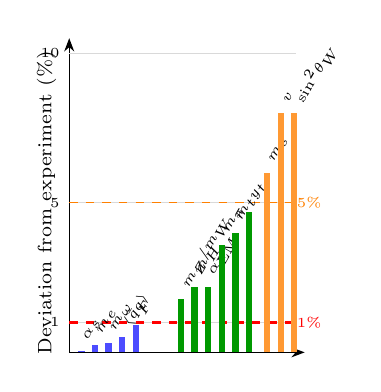
\begin{tikzpicture}[xscale=0.115, yscale=0.38]
 % Axes
 \draw[-{Stealth}] (0,0) -- (26,0);
 \draw[-{Stealth}] (0,0) -- (0,10.5);
 \node[rotate=90, font=\scriptsize] at (-2.5,5) {Deviation from experiment (\%)};

 % Grid lines
 \foreach \y in {1,5,10} {
 \draw[gray!30] (0,\y) -- (25,\y);
 \node[font=\tiny, left] at (0,\y) {\y};
 }

 % 1% line
 \draw[red, dashed, thick] (0,1) -- (25,1);
 \node[red, font=\tiny] at (26.5,1) {1\%};

 % 5% line
 \draw[orange, dashed] (0,5) -- (25,5);
 \node[orange, font=\tiny] at (26.5,5) {5\%};

 % Data bars (sorted by deviation)
 % <1%: me, pitau, mw, qq, msratio, NDelta, F
 \fill[blue!70] (1,0) rectangle (1.7,0.06); \node[font=\tiny,rotate=60,anchor=west] at (1.35,0.15) {$\alpha_s$};
 \fill[blue!70] (2.5,0) rectangle (3.2,0.24); \node[font=\tiny,rotate=60,anchor=west] at (2.85,0.35) {$m_e$};
 \fill[blue!70] (4,0) rectangle (4.7,0.32); \node[font=\tiny,rotate=60,anchor=west] at (4.35,0.45) {$m_\omega$};
 \fill[blue!70] (5.5,0) rectangle (6.2,0.5); \node[font=\tiny,rotate=60,anchor=west] at (5.85,0.6) {$\langle\bar qq\rangle$};
 \fill[blue!70] (7,0) rectangle (7.7,0.9); \node[font=\tiny,rotate=60,anchor=west] at (7.35,1.0) {$F$};

 % 1-5%
 \fill[green!60!black] (12,0) rectangle (12.7,1.8); \node[font=\tiny,rotate=60,anchor=west] at (12.35,1.9) {$m_Z/m_W$};
 \fill[green!60!black] (13.5,0) rectangle (14.2,2.2); \node[font=\tiny,rotate=60,anchor=west] at (13.85,2.3) {$m_H$};
 \fill[green!60!black] (15,0) rectangle (15.7,2.2); \node[font=\tiny,rotate=60,anchor=west] at (15.35,2.3) {$\alpha_{\rm EM}$};
 \fill[green!60!black] (16.5,0) rectangle (17.2,3.6); \node[font=\tiny,rotate=60,anchor=west] at (16.85,3.7) {$m_\pi$};
 \fill[green!60!black] (18,0) rectangle (18.7,4.0); \node[font=\tiny,rotate=60,anchor=west] at (18.35,4.1) {$m_t$};
 \fill[green!60!black] (19.5,0) rectangle (20.2,4.7); \node[font=\tiny,rotate=60,anchor=west] at (19.85,4.8) {$y_t$};

 % 5-10%
 \fill[orange!80] (21.5,0) rectangle (22.2,6); \node[font=\tiny,rotate=60,anchor=west] at (21.85,6.1) {$m_s$};
 \fill[orange!80] (23,0) rectangle (23.7,8); \node[font=\tiny,rotate=60,anchor=west] at (23.35,8.1) {$v$};
 \fill[orange!80] (24.5,0) rectangle (25.2,8); \node[font=\tiny,rotate=60,anchor=west] at (24.85,8.1) {$\sin^2\!\theta_W$};
\end{tikzpicture}
\caption{Deviation of ESFT predictions from experiment for 16 quantities
(truncated at 10\%; see Table~\ref{tab:predictions} for full list).
Blue: $<\!1\%$, green: $1$--$5\%$, orange: $5$--$10\%$.
All from two scales and zero additional parameters.}
\label{fig:deviations}
\end{figure}


%----------------------------------------------------------------------
\section{Summary and experimental tests}
%----------------------------------------------------------------------

Table~\ref{tab:predictions} collects all predictions. Several
features distinguish ESFT from the Standard Model:

(i)~The tree-level relation $m_\pi m_\tau^{(0)} = \sigma$
(Eq.~\ref{eq:pitau}), a consequence of XY amplitude--phase duality,
has no SM explanation.

(ii)~The lepton--quark complementarity $m_\mu \approx m_s$ and
$m_s/\bar{m}_q = \epsilon^{-2/N_c}$ (0.7\%) suggest generation
structure is governed by~$N_c$.

(iii)~The three-field BKT formula~(\ref{eq:F}) is testable in
condensed-matter systems.

(iv)~ESFT predicts gravitational variation of coupling constants,
suppressed by BKT topological protection in weak fields (consistent
with all null results) but potentially measurable at neutron-star
surfaces: $\Delta\alpha/\alpha \sim 5\times10^{-7}$, testable with
XRISM and Athena X-ray missions.

Limitations: the individual $u$--$d$ mass splitting, CKM mixing, CP
violation, and the number of generations are not addressed in this
Letter (see Refs.~\cite{PaperVII} for mass exponents and CKM
mixing).

\begin{table}[t]
\caption{ESFT predictions from two scales ($\Qoppa$, $\sqrt{\sigma}$)
and BKT $\eta=1/4$. No free parameters beyond~$\Qoppa$.}
\label{tab:predictions}
\begin{ruledtabular}
\begin{tabular}{lllr}
Quantity & Formula & ESFT & Dev.\\
\hline
\textbf{$m_e$} & \textbf{$\sigma/(2\pi\Lambda)$} & \textbf{0.510 MeV} & \textbf{0.2\%}\\
\textbf{$m_\omega$} & \textbf{$2M_Q(1\!+\!\alpha_s/2\pi)$} & \textbf{785 MeV} & \textbf{0.3\%}\\
\textbf{$\langle\bar qq\rangle^{1/3}$} & \textbf{$(\sqrt\sigma)^3/(2\pi)$} & \textbf{249 MeV} & \textbf{0.5\%}\\
$m_s/\bar m_q$ & $\epsilon^{-2/N_c}$ & 27.4 & 1.2\%\\
$\Delta m_{N\Delta}$ & $\sigma/(2M_Q)$ & 290 MeV & 1.2\%\\
\textbf{$F(\lambda/J\!=\!1)$} & \textbf{Wolff MC} & \textbf{1.265} & \textbf{---}\\
\hline
$m_Z/m_W$ & $2/\sqrt3$ & 1.155 & 1.8\%\\
$m_H$ & $\Lambda\epsilon^{-1/8}$ & 122 GeV & 2.3\%\\
$1/\alpha_{\rm EM}$ & lattice$\to$RG & 140 & 2.2\%\\
$m_\pi$ & $\sqrt\sigma\cdot\epsilon^{1/4}$ & 133 MeV & 3.9\%\\
$m_t$ & $\Lambda\epsilon^{-1/5}$ & 178 GeV & 2.8\%\\
\hline
$m_s$ & $\Lambda\epsilon^{4/3}$ & 88 MeV & 6\%\\
$m_\mu$ & $\Lambda\epsilon^{4/3}$ & 88 MeV & 17\%\\
$m_c$ & $\Lambda\epsilon^{4/5}$ & 1.24 GeV & 2.4\%\\
\textbf{$m_b$} & \textbf{$\Lambda\epsilon^{5/9}$} & \textbf{4.17 GeV} & \textbf{0.2\%}\\
$\bar m_q$ & $\sigma/\Lambda$ & 3.21 MeV & 7\%\\
$v$ & $\Lambda\epsilon^{-1/4}$ & 227 GeV & 8\%\\
$\sin^2\!\theta_W$ & $1/4$ & 0.250 & 8\%\\
$y_t$ & $\sqrt2\,\epsilon^{1/20}$ & 1.10 & 11\%\\
$m_\tau$ & Koide ($A_2$ geom.) & 1841 MeV & 3.6\%\\
$f_\pi$ & GOR$\times\!\sqrt{\pi/2}$ & 93.9 MeV & 1.0\%\\
$M_Q$ & $(\sqrt\sigma/2\pi)\ln(1/\epsilon)$ & 362 MeV & 16\%\\
$V_{\rm well}$ & Yukawa & $-61$ MeV & 22\%\\
$\rho_\Lambda$ & $H_0^2M_{\rm Pl}^2/(2\pi)^2$ & $2\!\times\!10^{-47}$ & $\sim$2$\times$\\
\end{tabular}
\end{ruledtabular}
\end{table}


%----------------------------------------------------------------------
\begin{acknowledgments}
All derivations, interpretations, and conclusions
are the sole responsibility of the author.
\end{acknowledgments}

\begin{thebibliography}{9}

\bibitem{PaperI}
 J.\,C.\,P.\ Won Ting,
 ``Topological soliton coherence scale: one parameter across seven
 physical domains,''
 Zenodo (2026), \href{https://doi.org/10.5281/zenodo.19154442}{10.5281/zenodo.19154442}.

\bibitem{PaperII}
 J.\,C.\,P.\ Won Ting,
 ``Emergent gauge symmetry from Hopf soliton topology in ESFT,''
 Zenodo (2026), \href{https://doi.org/10.5281/zenodo.19159255}{10.5281/zenodo.19159255}.

\bibitem{NK1977}
 D.\,R.\ Nelson and J.\,M.\ Kosterlitz,
 Phys.\ Rev.\ Lett.\ \textbf{39}, 1201 (1977).

\bibitem{KT1973}
 J.\,M.\ Kosterlitz and D.\,J.\ Thouless,
 J.\ Phys.\ C \textbf{6}, 1181 (1973).

\bibitem{Adams1960}
 J.\,F.\ Adams,
 Ann.\ Math.\ \textbf{72}, 20 (1960).

\bibitem{Witten1983}
 E.\ Witten,
 Commun.\ Math.\ Phys.\ \textbf{92}, 455 (1983).

\bibitem{FR1968}
 D.\ Finkelstein and J.\ Rubinstein,
 J.\ Math.\ Phys.\ \textbf{9}, 1762 (1968).

\bibitem{PDG2024}
 R.\,L.\ Workman \textit{et al.} (Particle Data Group),
 Prog.\ Theor.\ Exp.\ Phys.\ \textbf{2022}, 083C01.

\bibitem{FLAG2021}
 Y.\ Aoki \textit{et al.} (FLAG),
 Eur.\ Phys.\ J.\ C \textbf{82}, 869 (2022).

\bibitem{PaperVII}
 J.~C.~P.~Won Ting,
 ``Topological gauge modulation and Fibonacci structure of fermion
 masses in ESFT,''
 in preparation (2026).

\bibitem{Koide1983}
 Y.\ Koide,
 Phys.\ Lett.\ B \textbf{120}, 161 (1983).

\end{thebibliography}

\end{document}
